\documentclass[12pt]{article}
\usepackage[utf8]{inputenc}
\usepackage{graphicx}
\usepackage{caption}
\usepackage{algpseudocode}
\usepackage{algorithm}
\usepackage{algorithmic}
\usepackage{booktabs}
\usepackage{tabularx}
\usepackage{tabularray}
\usepackage{hyperref}

\hypersetup{
    colorlinks=true,
    linkcolor=blue,
    filecolor=magenta,      
    urlcolor=cyan,
    pdftitle={Overleaf Example},
    pdfpagemode=FullScreen,
    }

\urlstyle{same}
\title{Applicazione di un algoritmo genetico per la risoluzione del  Graph coloring problem}
\author{Salvatore Borgesi}
\date{Dicembre 2022/Gennaio 2023}

\begin{document}

\maketitle
\section{Introduzione}
\setcounter{page}{1}

Il problema da trattare consiste nel colorare i vertici di un grafo considerando un vincolo. Dato un numero di colori, vi è la necessità di colorare i vertici in maniera tale che due nodi adiacenti non abbiano lo stesso colore. 
Il numero minimo di colori che può essere utilizzato viene definito  \textbf{chromatic number} \chi(G). \end{chi} 
La risoluzione a questo problema può essere adottata in diversi contesti applicativi  quali:
\begin{enumerate}
    \item Scheduling.
    \item Gioco del Sudoku.
    \item Colorazione delle mappe.
\end{itemize}


\noindent La scelta dell'algoritmo genetico per il problema, è stata dettata dal fatto che essa mi consente di migliorare le soluzioni ottenute iterazione per iterazione e portando al successivo step solo le soluzioni che si "avvicinano" di più al raggiungimento dell' ottimo.

\section {Rappresentazione della popolazione iniziale}
Per l'inizializzazione della popolazione iniziale viene prima di tutto definito un vettore di interi che va da 1 fino al numero massimo di colori che si vuole utilizzare per colorare i vertici del grafo affinché venga rispettato il vincolo di colorazione del problema. Supponiamo dunque, che il numero di colori sia pari a n = 10. L'array che definisce i colori sarà:[1,2,3...,10]. Data quest'ultima lista, viene successivamente definita una soluzione (rappresentata anche essa da un'array) di lunghezza pari al numero di vertici del grafo. A ciascun cassetto della lista, viene assegnato in maniera casuale uno dei valori numerici definiti nell'arrray precedente. Questa operazione di generazione di un singolo individuo, viene eseguita ripetutamente fino a raggiungere il numero di individui desiderati (rappresentato in un file di configurazione tramite la variabile POPULATION\_SIZE).

\begin{algorithm}
\caption{Initialize Population}\label{alg:cap}
\begin{algorithmic} 
\State \While{$Population \leq POPULATION\_SIZE$}
    \State {$solution \gets [ ]$}
    \State {$colors \gets [1 ... StartColorSize]$}
        \For{\texttt{each vertex}}
            \State{$color \gets random(colors)$}
            \State{$solution[vertex] \gets $ color$}
        \endfor

\endwhile
\end{algorithmic}
\end{algorithm}

\section{Funzione di fitness}
In un algoritmo genetico, la funzione di fitness consente di comprendere quale tra K individui è il migliore e quindi andrà con una certa probabilità alle iterazioni successive. La fitness definita all'interno della soluzione costruita, esamina ciascun arco del grafo, e per ciascuno viene verificato se due nodi adiacenti hanno lo stesso colore. In caso di esito positivo viene aggiunta una penalità. Successivamente, la somma degli archi che collegano due vertici aventi lo stesso colore, viene moltiplicata per il numero di colori che sta utilizzando la soluzione valutata. Questo prodotto perciò, restituisce zero se tutti i vertici sono colorati in maniera corretta, rispettando i vincoli del problema. Dopo diversi esperimenti ho notato che questa prima "versione" di valutazione ad un determinato punto non riusciva più a migliorare poiché se l'algoritmo trovava due soluzioni con fitness pari a zero, non riusciva a capire quale delle due soluzioni era la migliore. Questo perché, nonostante le soluzioni erano entrambe valide, una di esse potenzialmente poteva avere un valore cromatico più basso. Proprio per tale motivo ho deciso di aggiungere al prodotto citato prima, il numero di colori utilizzato. Facendo un esempio si supponga di avere due soluzioni corrette nella quale la prima ha 5 colori, invece la seconda ne ha 6. Con la seconda funzione di fitness descritta, nonostante le due soluzioni siano entrambe corrette, la prima sarà migliore in quanto utilizza un minor numero di colori per il grafo.

\begin{algorithm}
\caption{Fitness function}\label{alg:cap}
\begin{algorithmic} 
    \State {$count \gets 0$}
    \State {$colors \gets numero\ di\ colori\ usati\ dalla\ soluzione$}
        \For{\texttt{each edges}}
            \If{$colore\ vertice\ u == colore\ vertice\ v $} 
            \State $count \gets count+1$
            \EndIf
        \EndFor
    \State \textbf{return} $(colors * count) + colors$}
\end{algorithmic}
\end{algorithm}

\section{Algoritmo utilizzato e pseudocodice}
In questa sezione della relazione scenderò più nel dettaglio nell'esaminare e descrivere l'algoritmo costruito per la risoluzione del problema.

\begin{algorithm}
\caption{Genetic algorithm}\label{alg:cap}
\begin{algorithmic} 
    \State{$graph \gets TranslateDimacsInstance()$}
    \State {$Population \gets InitializePopulation(graph)$}
    \State {$ColoreIniziale \gets Getupperbound(graph)$} 
    \State {$fitnessCount \gets 0$}
    \While {$ not\  Stopping \ criteria $}
    \State {$nuovaPopolazione\gets []$}
        \For{\texttt {i to POPULATION\_\ SIZE/2}}
            \State{$Selection();$}
            \State{$Crossover();$}
            \State{$Mutation();$}
            \State{$Replacement();$}

            \If{$FitnessAbsoluteBestSolution \geq ActualBestSolution$} 
                \State{$FitnessAbsoluteBestSolution \gets ActualBestSolution$}
            \EndIf
            \If{$fitnessCount > MAX\_\ NUMERO \_\ VALUTAZIONI$}
                \State{$StoppingCriteria \gets True$} 
\end{algorithmic}
\end{algorithm}



\noindent Come descritto  sopra, la prima parte consiste nel tradurre le istanze fornite nel formato \textit{.col} in maniera tale da poter essere rappresentate mediante codice. Per far questo sono state definite due classi: \textit{Graph()} e \textit{Vertex()}. All'interno dell'oggetto grafo saranno presenti la lista di archi e la lista di vertici. Ogni oggetto vertice tiene traccia di chi sono i nodi adiacenti ad esso.


\noindent Lo pseudocodice, evidenzia come le operazioni più importanti siano quelle di \textit{Selection}, \textit{Crossover}, \textit{Mutation} e di \textit{Replacement} che stanno alla base del funzionamento di un algoritmo genetico. Dopo aver generato la popolazione iniziale, viene determinato mediante il metodo \textit{GetUpperbound()} qual'è il colore con la quale si inizierà a 'dipingere' i nodi del grafo. Questo metodo banalmente, prende come riferimento il numero di archi uscenti per ciascun vertice e ne restituisce il valore più alto . L'algoritmo si conclude quando è stato raggiunto il numero massimo di valutazioni. Qualora  il valore della funzione obiettivo  è più vantaggioso di un altro (e la soluzione risulta valida) , viene sostituita la AbsoluteBestFitness precedente con quella appena trovata.

\subsection{Selection}
Il processo di \textit{Selezione} consiste nel selezionare tra la popolazione generata nella fase di inizializzazione la "\textit{prole}" che sarà portata avanti nelle successive generazioni. In questo progetto sono state implementate tre tipi di operatori di selezione.

\subsubsection{Roulette}

Tramite questa modalità di selezione, vengono selezionati con probabilità più alta i genitori che hanno una fitness migliore. Per come è stata calcolata la fitness in questo progetto, i genitori che hanno un valore di fitness basso, avranno una maggiore probabilità di essere selezionati.

\subsubsection{Random}
Questa strategia prevede una selezione casuale dei genitori. 

\subsubsection{Tournament}
Con l'utilizzo di questa strategia vengono estratti K individui dalla popolazione. Di questi K individui, viene selezionato quello che detiene il valore di fitness migliore.

\subsubsection{Strategia adottata per la selezione}
Mentre i tre metodi sopra citati sono stati tutti implementati nel codice, la decisione finale è stata quella di utilizzare la modalità \textit{Tournament} con un valore di K = 20. L'utilizzo di questo operatore infatti, consente anche a configurazioni non ottimali di fare parte delle future generazioni, dando l'opportunità di spaziare tra differenti soluzioni e non convergere dunque in un ottimo locale. Sono stati effettuati diversi tentativi, ad esempio con con K = 10. Con quest'ultimo infatti, ho notato che anche se l'algoritmo arriva a convergenza più velocemente, rischia dopo diverse iterazioni di rimanere bloccato in un punto di ottimo locale.

\section{Crossover}
L'operatore genetico di crossover offre l'opportunità di mescolare le soluzioni ottenute mediante l'operatore di selezione ed ottenere perciò dei nuovi figli. Gli operatori di crossover sviluppati durante la realizzazione del prodotto sono il \textit{Single one-point crossover} e il \textit{Two-point crossover}.

\subsection{Single one-point crossover}
Dai figli generati durante la fase di Selezione, viene selezionato in modo tutto casuale un punto che ci consentirà di tagliare la lista in due parti e di effettuarne uno scambio.

\begin{center}
\includegraphics[width=0.5\textwidth]{images/one_point_crossover.png}
\end{center}
\subsection{Two-point crossover}
In questo caso, invece di selezionare un unico punto di taglio, vengono scelti due punti (randomici) delle due liste e vengono successivamente mischiate le due stringhe.

\begin{center}
\includegraphics[width=0.5\textwidth]{images/two_point_crossover.png}
\end{center}
\subsection{Stratgia adottata per il crossover}

Inizialmente, nella realizzazione del progetto ho utilizzato il single one-point crossover con una probabilità di 0.9. Ho notato tuttavia, che utilizzare il 2-point crossover anche se con una probabilità più bassa (0.8) riesce ad apportare delle modifiche alle soluzioni generate e per tale motivo è stata mantenuta tale scelta per gli esperimenti. 


\section{Mutation}
L'operazione di mutazione, dato un cromosoma, consente di variarne un 'gene' ottenendo come conseguenza una nuova soluzione. Per questo progetto sono state sviluppate due varianti.

\subsection{Random mutation}
Rappresenta l'operazione di mutazione più semplice. In breve, viene selezionato un elemento del cromosoma, viene selezionato un colore (in maniera casuale), e quest'ultimo (il colore) viene assegnato all'elemento scelto durante la prima fase.

\begin{algorithm}
\caption{Random mutation}\label{alg:cap}
\begin{algorithmic} 
    \State {$posizioneDaModificare \gets random(1,numeroVertici)$}
    \State {$ numeroColori \gets numeroColoriPresentiNellaSoluzione$}
    \State {$soluzione[posizioneDaModificare] \gets random(1,numeroColori)$} 
   
    
\end{algorithmic}
\end{algorithm}


\subsection{Vertex mutation}
Questo tipo di mutazione è stata costruita per risolvere il problema assegnato. 

\begin{algorithm}
\caption{Vertex mutation}\label{alg:cap}
\begin{algorithmic} 
    \State {$ColoriModificati \gets 0$} 
        \For{\texttt {vertex \textbf{in} Vertices}}
            \State{$neighbors \gets vertex.getNeighbors()$}
             \For{\texttt {neighbor in Neighbors}}
                \If{$solution[vertex] == solution[neighbor]$}
                    \State{$solution[vertex] \gets random(1,numeroColoriUsatiDallaSoluzione)$}
                    \State{$coloriModificati \gets coloriModificati + 1$}
                \EndIf
             \EndFor
        \EndFor
    \If{$ColoriModificati == 0$}
        \State{$posDaModificare  \gets random(1,numeroVertici)$}
        \State{$posCasuale  \gets random(1,numeroVertici)$}
          \If{$colorePosizioneDaModifcare == colorePosizioneCasuale$}
            \State{$colorePosizioneDaModificare \gets random(1,arrayColori)$}
          \Else
            \State{$colorePosizioneDaModificare \gets colorePosizioneCasuale$}
          \EndIf
\end{algorithmic}
\end{algorithm}


\noindent Per ciascun vertice, viene recuperata e ciclata la lista dei suoi nodi adiacenti. Dunque, per ciascun 'vicino' viene effettuato un controllo ovvero se il vertice e i vicini hanno lo stesso colore. In caso di esito positivo viene assegnato randomicamente un colore in un range che va da 1 al numero massimo di colori utilizzati in quell'istante dalla soluzione. Inoltre, viene incrementato un contatore che identifica il numero di colori che sono stati modificati. Dopo aver esaminato ciascun vertice ed il proprio vicinato, se risulta che durante le iterazioni non è stato modificato nessun colore, vuol dire che la soluzione è valida e di conseguenza si sceglierà in maniera casuale una posizione della soluzione alla quale sarà assegnato un colore diverso. Questa seconda parte del codice è stata introdotta poiché senza di essa, dopo un discreto numero di iterazioni, gli individui ottenuti si fossilizzavano in un ottimo locale non andando a decrementare il numero di colori utilizzato.



\subsection{Strategie adottate per la Mutation}
Per alcune istanze , sono stati condotti degli esperimenti sia applicando la random mutation che la "Vertex mutation" sviluppata ad Hoc con alcuni accorgimenti legati alla rappresentazione del problema. 

\begin{center}
\includegraphics[width=1\textwidth]{images/colors_.png}
\end{center}

Il grafico in figura mostra un esempio di due iterazioni dove linea azzurra rappresenta l'andamento del numero di colori in funzione delle valutazioni effettuate utilizzando la random mutation mentre, la linea grigia,  mostra l'andamento per la vertex mutation. Si può facilmente notare che per quest'ultimo, il numero di colori converge più velocemente e inoltre raggiunge un valore più basso rispetto al primo caso. Ulteriori aspetti e considerazioni saranno considerate nella parte legata ai risultati ottenuti.

\section{Replacement}
Questa fase consente di sostituire la popolazione. Fondamentalmente sono state utilizzate due tipi di replacement.  La prima è la \begin  + \mu + \lambda \ replacement  \end   ..  Questa soluzione mette insieme la popolazione attuale con quella appena generata. La nuova popolazione dunque sarà formata dagli individui che presentano il valore di fitness più basso. Questo replacement avviene con una certa probabilità (impostata dal file di configurazione a 0.2). Altrimenti la popolazione appena costruita rimpiazzerà totalmente la popolazione precedente .

\section{Struttura del progetto}
Il progetto è stato realizzato utilizzando Python. La struttura data è la seguente:
\begin{itemize}
    \item \textit{instances}: contiene tutte le istanze dimacs da utilizzare
    \item \textit{logs} : contiene i grafici sia con le prove effettuate con la vertex mutation che con la random mutation.
    \item \textit{src}: codice sorgente.
    \item \textit{results}: risultati di ciascuna iterazione. In particolare per ciascuna istanza è stato generato un file contenente diverse informazioni quali Best color, Mean color , Std , Tempo di esecuzione.
    \item \textit{result vertex mutation}: Risultati con l'utilizzo della vertex mutation.
\end{itemize}

\noindent Ulteriori informazioni riguardanti l'installazione e l'esecuzione del codice sono disponibili alla pagina \href{https://github.com/borgesis95/GCP-with-Genetic-algorithm} {github} .


    

\section{Risultati ottenuti e conclusioni}

Sono stati realizzati due esperimenti ove la modifica più sostanziale è stato l'utilizzo nel primo caso della mutazione random, mentre nel secondo caso è stata utilizzata la Vertex mutation. In tabella vengono riportati alcuni dei valori del primo esperimento:




\begin{table}[htbp]
\begin{center}
\begin{tabular}{|l|l|l|l|l|} 
 \toprule Nome istanza  & Miglior colore & Media & Std  & Tempo di esecuzione \\ 
\midrule
queen5\_5.col  & 5              & 6.8   & 0.74 & 28m                 \\ 
queen6\_6.col  & 8              & 9.1   & 0.7  & 41m                 \\ 
queen7\_7.col  & 10             & 10 & 0 & 53m          \\ 
queen8\_8.col  & 14             & 14.2  & 0.39 & 1h and 30m          \\ 
queen8\_12.col & 18             & 19.3  & 0.89 & 3h and 12m          \\ 
queen9\_9.col & 14             & 15.1  & 0.53 & 2h and 14m          \\ 
DSJC125\_1.col & 12             & 12.4  & 0.6 & 347m       \\ 
DSJC125\_5.col & 27             & 28.5  & 0.89 & 2h and 1m      \\ 
DSJC125\_9.col & 52             & 52.9  & 1.13 & 4h and 16m      \\ 
le450\_15b.col & 40             & 42.4  & 2.09 & 4h and 40m      \\ 
le450\_15c.col & 57             & 60.4  & 2.28 & 8h and 54m      \\ 
le450\_15d.col & 56             & 59  & 2.36 & 8h and 48m      \\ 
\bottomrule
\end{tabular}
\caption{\label{table:tabella1}Risultati ottenuti con la random mutation}
\end{center}
\end{table}

\noindent I risultati della tabella ci danno alcune informazioni di cui vale la pena confrontare con la tabella \ref{table:tabella2}  che rappresenta invece gli esperimenti (di tutte le istanze assegnate) effettuati con la vertex mutation:


\begin{table}[htbp]
\begin{center}
\begin{tabular}{|l|l|l|l|l|} 
 \toprule Nome istanza  & Miglior colore & Media & Std  & Tempo di esecuzione \\ 
\midrule
queen5\_5.col  & 5              & 5   & 0 & 24m                 \\ 
queen6\_6.col  & 8              & 8   & 0  & 37m                 \\ 
queen7\_7.col  & 10             & 10.1  & 0.3 & 53m           \\ 
queen8\_8.col  & 12             & 12.8  & 0.4 & 1h and 19m          \\ 
queen8\_12.col & 17             & 18.2  & 0.6 & 2h and 18m          \\ 
queen9\_9.col & 15             & 15.8  & 0.4 & 1h and 48m  \\ 
DSJC125\_1.col & 11             & 12.3  & 0.64 & 50m      \\ 
DSJC125\_5.col & 27             & 28.9  & 0.83 & 3h and 7m      \\ 
DSJC125\_9.col & 52             & 53.3  & 0.78 & 4h and 50m      \\ 
le450\_15b.col & 47             & 50.2  & 1.53 & 7h and 33m      \\ 
le450\_15c.col & 61             & 64.3  & 1.9 & 18h and 37m \\ 
le450\_15d.col & 63             & 65.5  & 2.06 & 1day and 10h      \\ 


\bottomrule
\end{tabular}
\caption{\label{table:tabella2} Risultati ottenuti con la vertex mutation}
\end{center}
\end{table}

 \noindent Confrontando le due tabelle si può notare come nelle istanze più piccole il miglior valore cromatico dei grafi è uguale, tuttavia si osservi che non in tutte le iterazioni (runs) viene ottenuto sempre lo stesso valore. Questo è deducibile dai valori della media. Nelle istanze di medie dimensioni (queen8\_8.col e 8\_12.col) nella tabella \ref{table:tabella1} si nota come il numero di colori utilizzati per colorare il grafo è più basso (così come la media). Osservando infine le istanze più grandi, nonostante il numero di colori utilizzato per ciascuna valutazione diminuisce in modo più deciso utilizzando la vertex mutation, i risultati ottenuti mutando in modo casuale il colore dei vertici sono migliori. 




\begin{figure}[H]
\caption{linea azzurra:  Random mutation - linea blu : Vertex mutation}
\centering
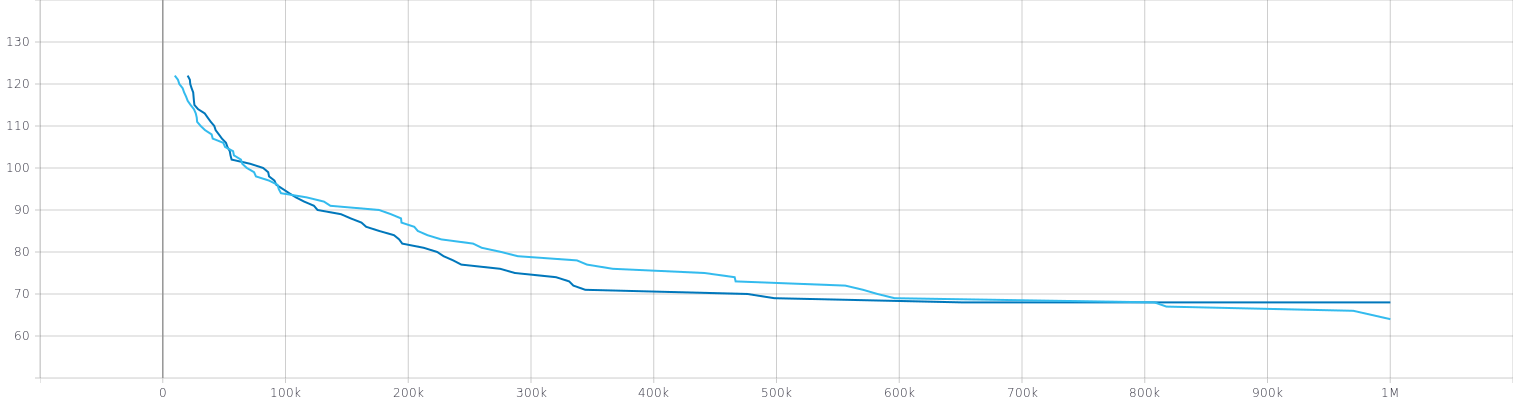
\includegraphics[width=1\textwidth]{images/le450d.png}
\end{figure}

\noindent La figura sovrastante mostra come nel caso del grafo \textit{le450\_15d.col} la vertex mutation converge più velocemente, tuttavia alla fine delle valutazioni essa utilizzerà un numero maggiore di colori rispetto alla random mutation.

\begin{figure}[H]
\caption{linea azzurra:  Vertex mutation - linea arancione : Random mutation}
\centering
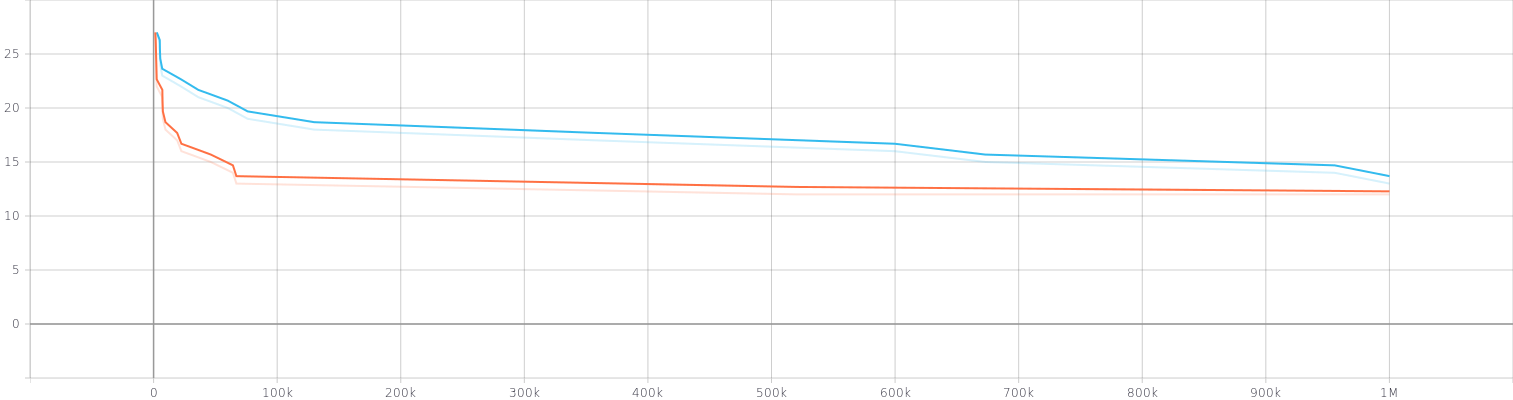
\includegraphics[width=1\textwidth]{images/queen8_8.png}
\end{figure}

\noindent Da questo grafico (che rappresenta il comportamento per l'istanza queen8\_8.col) può essere dimostrato come nel caso di istanze medie la "vertex mutation" non solo converge prima ma (generalmente), riesce a colorare il grafo con un numero più basso di colori rispetto alla random mutation. 
Come descritto nella documentazione \href{https://github.com/borgesis95/GCP-with-Genetic-algorithm} {github}, del progetto, è possibile vedere i grafici di ciascuna istanza (sia per la random che per la vertex mutation), lanciando il comando  \textit{tensorboard --logdir logs}.



\section{Conclusioni}
Dai vari esperimenti e dall' approfondimento di questa famiglia di algoritmi si può notare come risultano fondamentali due caratteristiche:
\begin{itemize}
  \item Il tempo di esecuzione
  \item Il risultato ottenuto
\end{itemize}

\noindent Inoltre è essenziale conoscere ed approfondire le peculiarità del problema che si sta provando ad affrontare. Con tale conoscenza infatti, è possibile costruire degli operatori ad hoc che hanno il doppio compito di trovare la soluzione migliore e di non bloccarsi in un ottimo locale. Un implementazione futura, data anche la natura del problema potrebbe essere quella di adottare un approccio ibrido utilizzando una local search.  Il tempo di esecuzione inoltre, ha inciso in maniera non indifferente, dunque sarebbe opportuno ottimizzare il codice creato o utilizzare un linguaggio più performante come C++.

\end{document}

